\documentclass[border=3pt]{standalone}
% Preâmbulo compartilhado pelos diagramas TikZ da aula 8 de IHR (Métodos de Pesquisa)
\usepackage[T1]{fontenc}
\usepackage[utf8]{inputenc}
\usepackage{lmodern}
\usepackage{amsmath}
\usepackage{xcolor}
\usepackage{tikz}
\usetikzlibrary{arrows.meta,angles,quotes,decorations.pathmorphing,decorations.pathreplacing,calc,
                positioning,shapes.geometric,shapes.misc,backgrounds,fit,
                math}

% Paleta (mesma dos SVGs originais)
% Paleta da disciplina de IHR: acento azul (#1A6FB5), cor de destaque do tema.
% (o nome "dblue" é mantido para não alterar todos os diagramas)
\definecolor{dblue}{HTML}{1A6FB5}
\definecolor{dorange}{HTML}{B3541E}
\definecolor{dgreen}{HTML}{4A7C59}
\definecolor{dred}{HTML}{9C4B4B}
\definecolor{dcream}{HTML}{F4F1EA}
\definecolor{dshade}{HTML}{DDD7C9}

% Função gaussiana (não normalizada por padrão de escala visual)
\pgfmathdeclarefunction{gauss}{3}{%
  \pgfmathparse{1/(#3*sqrt(2*pi))*exp(-((#1-#2)^2)/(2*#3^2))}%
}

% Estilos comuns (prefixo d... para não colidir com chaves internas do pgf)
\tikzset{
  >={Stealth[length=2mm]},
  dguide/.style={gray!55, dashed, line width=0.4pt},
  daxis/.style={gray!60, line width=0.7pt, ->},
  dbody/.style={fill=black!3, draw=black!80, line width=1pt},
  dacc/.style={draw=dblue, line width=1pt},
  dlbl/.style={black!55, font=\small},
  dsub/.style={black!45, font=\footnotesize},
  dstate/.style={circle, draw=black!80, fill=dcream, line width=1pt,
                 minimum size=17mm, font=\large, inner sep=1pt},
  dobs/.style={circle, draw=black!80, fill=dshade, line width=1pt,
               minimum size=14mm, font=\large, inner sep=1pt},
  dbox/.style={rounded corners=2pt, draw=black!80, fill=dcream, line width=1pt,
               align=center, inner sep=6pt},
  dop/.style={circle, draw=black!80, fill=white, line width=1pt,
              minimum size=6mm, inner sep=0pt, font=\small},
  dtrans/.style={->, dblue, line width=1pt},
  dmeas/.style={->, dorange, line width=1pt},
  dcurve/.style={line width=1pt, dblue},
  dcurveb/.style={line width=1.4pt, dorange},
}

\begin{document}
\hyphenpenalty=10000 \exhyphenpenalty=10000 \tolerance=9999 \emergencystretch=3em
\newcommand{\pess}[3]{% x, y, cor
  \draw[#3, fill=#3!15, line width=1.3pt] (#1,#2+0.42) circle (0.28);
  \draw[#3, fill=#3!15, line width=1.3pt, rounded corners=4pt] (#1-0.5,#2-0.65) rectangle (#1+0.5,#2+0.05);}
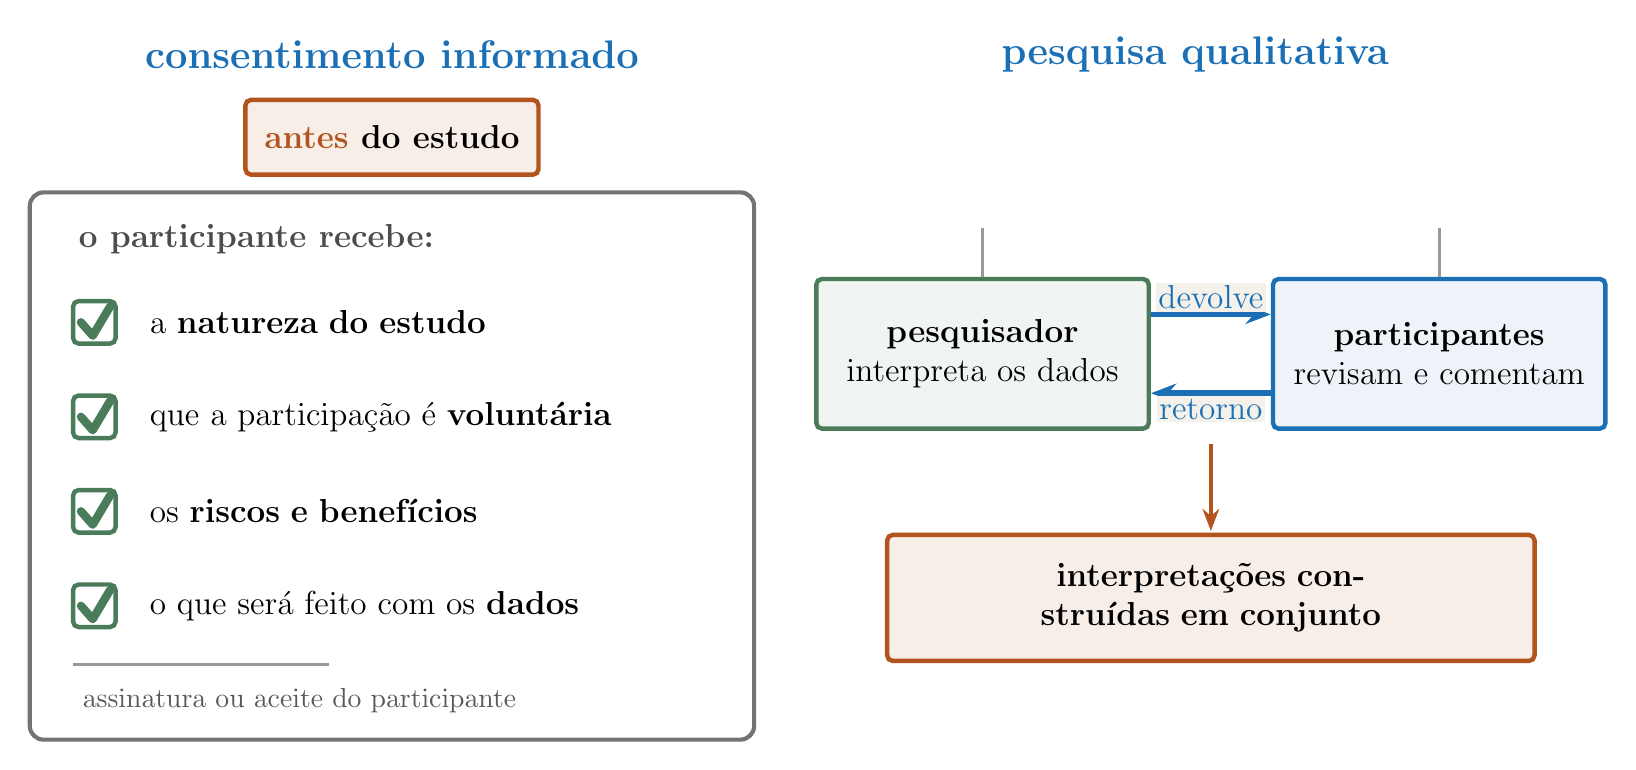
\begin{tikzpicture}[x=1cm,y=1cm]
  \tikzset{item/.style={font=\large, anchor=west, text width=6.4cm}}
  % ---------- painel esquerdo: consentimento antes ----------
  \node[font=\Large\bfseries, dblue] at (5.0,9.4) {consentimento informado};
  \node[dbox, draw=dorange, fill=dorange!10, line width=1.6pt, text width=3.3cm, minimum height=0.95cm, font=\large\bfseries] at (5.0,8.35) {\textcolor{dorange}{antes} do estudo};
  \draw[black!55, fill=white, line width=1.5pt, rounded corners=5pt] (0.4,0.7) rectangle (9.6,7.65);
  \node[font=\large\bfseries, black!70, anchor=west] at (0.9,7.05) {o participante recebe:};
  \foreach \y/\t in {6.0/{a \textbf{natureza do estudo}}, 4.8/{que a participação é \textbf{voluntária}}, 3.6/{os \textbf{riscos e benefícios}}, 2.4/{o que será feito com os \textbf{dados}}} {
    \draw[dgreen, line width=1.6pt, rounded corners=2pt] (0.95,\y-0.27) rectangle ++(0.54,0.54);
    \draw[dgreen, line width=3pt, line cap=round, line join=round] (1.05,\y) -- (1.2,\y-0.17) -- (1.42,\y+0.2);
    \node[item] at (1.8,\y) {\t};
  }
  \draw[black!40, line width=1pt] (0.95,1.65) -- (4.2,1.65);
  \node[font=\normalsize, black!65, anchor=west] at (0.95,1.2) {assinatura ou aceite do participante};
  % ---------- painel direito: devolver resultados ----------
  \node[font=\Large\bfseries, dblue] at (15.2,9.4) {pesquisa qualitativa};
  \node[dbox, draw=dgreen, fill=dgreen!8, line width=1.6pt, text width=3.8cm, minimum height=1.9cm, font=\large, align=center] (p) at (12.5,5.6) {\textbf{pesquisador}\\ interpreta os dados};
  \node[dbox, draw=dblue, fill=dblue!8, line width=1.6pt, text width=3.8cm, minimum height=1.9cm, font=\large, align=center] (q) at (18.3,5.6) {\textbf{participantes}\\ revisam e comentam};
  \draw[dtrans, line width=2pt, -{Stealth[length=3.2mm]}] ([yshift=0.5cm]p.east) -- node[above, font=\large, fill=dcream, inner sep=1pt] {devolve} ([yshift=0.5cm]q.west);
  \draw[dtrans, line width=2pt, -{Stealth[length=3.2mm]}] ([yshift=-0.5cm]q.west) -- node[below, font=\large, fill=dcream, inner sep=1pt] {retorno} ([yshift=-0.5cm]p.east);
  \node[dbox, draw=dorange, fill=dorange!10, line width=1.6pt, text width=7.8cm, minimum height=1.6cm, font=\large, align=center] at (15.4,2.5) {\textbf{interpretações construídas em conjunto}};
  \draw[dorange, line width=1.6pt, -{Stealth[length=2.8mm]}] (15.4,4.45) -- (15.4,3.35);
  \pess{12.5}{8.0}{dgreen} \pess{18.3}{8.0}{dblue}
  \draw[black!40, line width=1pt] (12.5,7.2) -- (p.north); \draw[black!40, line width=1pt] (18.3,7.2) -- (q.north);
\end{tikzpicture}
\end{document}
